\documentclass{article}
\usepackage{fullpage}
\usepackage{graphicx}
\begin{document}
    \title{Behaviors: An Introduction and Exercises}
    \author{Russell Cohen}
    \date{\today}
    \maketitle
    \section{What is a behavior?}
    At its most basic, a behavior is machine with two input terminals and two
    output terminals.  One of these input terminals is external input.  The
    other is feedback from the behavior.  Similarly, the behavior has two output
    terminals.  One gets released externally as output, and the other gets fed
    back to the behavior.  At their core, behaviors have nothing to do with
    pixels are light effects -- this is merely how we commonly use them.
    \begin{center}
    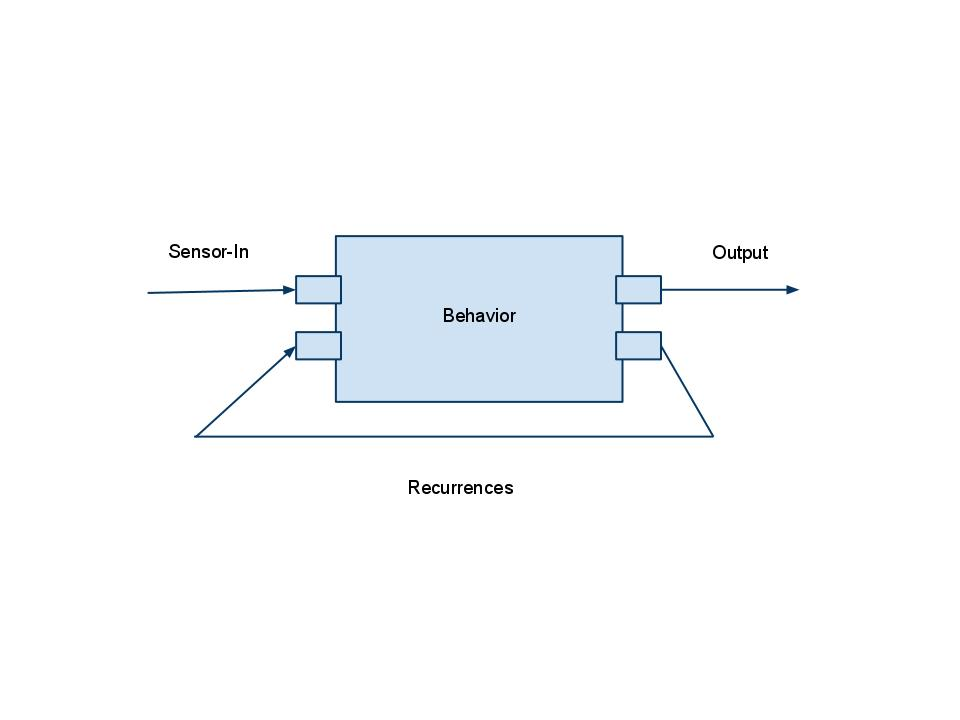
\includegraphics[width=4 in]{Behavior.jpg}
    \end{center}
    \section{How do I write a behavior?}
    At the core of a behavior is its \texttt{ProcessResponse} method which
    tells a behavior what to get on input.  As you might expect, it has 2
    input ports, and two output ports.  The `type' of inputs and outputs can be
    anything -- numbers, strings, lists, however, in our system, the inputs
    and outputs are all python dictionaries.  This allows us to have an
    arbitrary number of named parameters.  As sample input might look
    something like \texttt{{'Location':(20,20), 'Height':10}}.  When we
    return a value, we return a tuple of \texttt{(list<dict>,list<dict>)}.  Note that on a
    process response method you will actually be given a \textbf{List of
        dictionaries} and you should iterate over them. 
    \textbf{Important:} You should not directly modify the inputs!  Use
    \texttt{dict(input)} to create a copy of them!
    \section{Exercise 1: addFive}
    Our goal: Create a behavior that will add 5 to the 'Value' field of the
    input.  If no 'Value' field exists, we will set it to five.  Below is a
    sample \verb processResponse  method to do this.  Note that process
    response is the only part of a behavior that must be written (everything
            else happens behind the scenes when you \textbf{inherit} from the
            \texttt{Behavior} class.
    \begin{verbatim}
        def processResponse(self, inputs, recurrences):
            output = [] #empty list 
            for inp in inputs:
                inpCopy = dict(inp)
                if not ('Value' in inpCopy):
                    inpCopy['Value'] = 0
                inpCopy['Value'] += 5
                output.append(inpCopy)
            return (output, []) #empty list, no recurrences
    \end{verbatim}
    \section{Exercise 2: A Sum-er}
        Create a behavior that outputs the sum of all previous input.  Hint:
        You will need to use recurrences!
    \section{Declaring and Configuring Behaviors}
        Once you've written your behavior (or are using an already written
            behavior, you will need to tell the light installation to use the
            behavior.  This is done via XML in the configuration file.  When you
            run the system, you specify a configuration file eg:
            \texttt{python LightInstallation.py config/ConfigFile.xml}

            Behaviors are specified in the \verb BehaviorConfiguration  section.
            A sample behavior follows:
           \begin{verbatim}
            <Behavior>
                <Class>behaviors.EchoBehavior</Class>
                <Args>
                    <Id>echo</Id>
                    <RenderToScreen>False</RenderToScreen>
                </Args>
            </Behavior>
            \end{verbatim}

            The ``Class'' attribute specifies the \textbf{Python} class for this
            behavior.  (The \verb behaviors.  prefix tells Python to look in the
                behaviors folder).  You may recall that all classes SmootLight take a
            single python dictionary as an argument -- this is embodied by the
            \texttt{Args} tag.  A dictionary is created from the XML at runtime
            -- this dictionary would be: \texttt{{'Id':'echo',
                'RenderToScreen':False}}
            The id we specify is the id that we can reference this behavior by
            later.  The \verb RenderToScreen  attribute specifies whether or not
            outputs from this behavior should be directed to the screen (some
                    behaviors act only as the building blocks for other
                    behaviors, and are never rendered directly to the screen)

    \section{Behavior Chains}
        I have mentioned several times that the system allows for behaviors to
        be chained together to create many different effects -- often the
        ``motion'' effect and the ``coloring'' effects are two separate
        behaviors.  The result you see on the screen are these two pieces
        connected together.  This allows us to build up many different behaviors
        from a library of simple pieces.  Let's look at how we actually
        accomplish this.
        
        Behavior Chaining is accomplished through the behavior chain class.
        Here is an example of a behavior we declare (in XML) via a behavior
        chain:
        \begin{verbatim}
        <Behavior>
            <Class>behaviors.BehaviorChain</Class>
            <Args>
                <Id>runcolordecay</Id>
                <Inputs>
                    <Id>pygame</Id>
                    <Id>randomLoc</Id>
                </Inputs>
                <ChainedBehaviors>
                    <Id>colorchange</Id>
                    <Id>running</Id>
                    <Id>decay</Id>
                </ChainedBehaviors>
                <RecursiveHooks>{'running':'acceleratedie'}</RecursiveHooks>
                <RenderToScreen>True</RenderToScreen>
                <Mapper>gaussmap</Mapper>
            </Args>
        </Behavior>
        \end{verbatim}

        Note the importance of the `Id' field -- that is how we reference all
        other components of the system.  Let's walk through what is going on
        here.  We declare this behavior just like any other -- however, for
        class, we specify \verb BehaviorChain .  The \verb Inputs  tag specifies
        which inputs will be routed to this behavior.  In this case, it is
        \verb pygame  and \verb randomLoc  , two previously declared behaviors.
        Inputs from these behaviors will be passed to the behavior chain via
        sensorInputs.  Next, we have the meet of this chain, the behaviors it is
        composed of.  This states that first, an input is routed through
        \texttt{colorchange}.  \verb colorchange adds a color field to the
        sensor data.  Next, the input is routed to \verb running  a behavior
        that makes pixels run back and forth.  Finally, the input is routed to
        \verb decay  , a behavior that adds a decay ``PixelEvent'' that makes
        individual pixels turn on and then decay.

        The next item we see is \verb RecursiveHooks  .  This is a special
        feature of the \verb BehaviorChain  that allows us to augment the
        reccurences recursive events have.  We specify that we will augment the
        recursive behavior of \verb running  with another behavior, 
        \verb acceleratedie  which modifies increases the speed of the running
        behavior, and stops the behavior after a certain number of iterations.
        Note that recursive hooks take data in via their \textbf{external input}
        port, and \textbf{not} their recursive port.
        \begin{center} 
        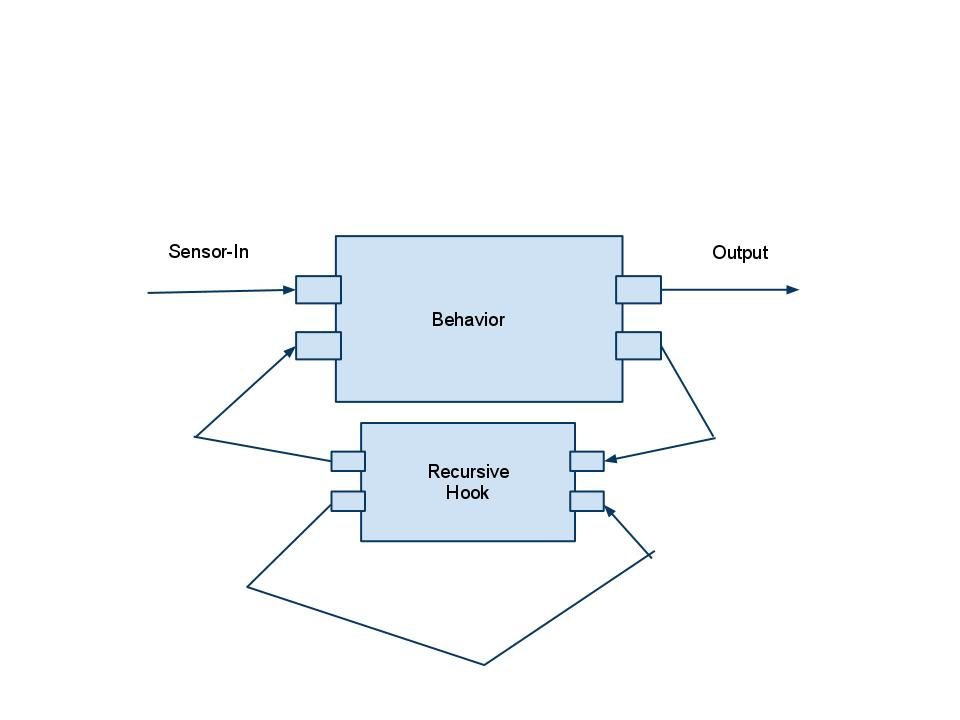
\includegraphics[width=4 in]{BehaviorwithRecursiveHook.jpg}
        \end{center}
        Finally, we state that this behavior will indeed be rendered directly to
        the screen, by specifying:
        \begin{center}\texttt{<RenderToScreen>True</RenderToScreen>} \end{center}
        We also specify which PixelMapper we want to use (gaussmap):
        \texttt{<Mapper>gaussmap</Map>}.  \verb gaussmap  is the id we assigned to the mapper when
        we declared in the \verb PixelMappers  section of the xml.
        \begin{center}
        Phew.  This isn't as complicated as it sounds.  I promise.
        \end{center}
        Browse around the behaviors to get an idea of what is possible and what has been done.  They
        all live in the behaviors folder.  Enjoy!
        \end{document}
